\input{../../../Skript_praeambel.tex}

% !TeX spellcheck = en_US 

\begin{document}
%Ben�tigte Angaben f�r die Titelseite
\title{Summary of the lecture \\ \glqq MA INF 4316 - Graph Representation Learning\grqq\! \\ by Dr. Pascal Welke \\ (WiSe 2021/2022)}
%Hier Zeilenumbruch durch \\, da \newline in dieser Umgebung nicht funktioniert.
\author{Fabrice Beaumont \\ Matrikel-Nr: 2747609 \\
Rheinische Friedrich-Wilhelms-Universit�t Bonn}

%Erstellung des Titels
\maketitle
\tableofcontents
%\listoffigures

%----------------------------------------------------------

%TODO Remarks:
% Lec 0: Slide 7/38 - "focus ON the following questions"
% Lec 0: Slide 20/38 - "additionally contain INformation about"
% Lec 0: Slide 26/38 - "Decision Trees, and Random Forests" - Also this time the methods are writen with capitalized letters. Earler they were not. (Also not all of them were listed.)
% Lec 0: Slide 31 vs slide 33- In the vertex classification example the data-consistent hypothesis is presented as THE correct solution. In the graph classifiaction the presented one is suggested to fit the example. I personally think the later formulation is better.
% Lec 0: Slide 33/38 - "graphs of THE blue class"

% Lec 1: Slide 10/54 - Using "vertices", but previously "nodes"
% Lec 1: Slide 10/54 - So simple graphs can have loop-edges? e={v, v} \in E
% Lec 1: Slide 16+17/54 - The loss function for vertex property prediction is given as L_{G,y} but later on slide 20 and the following as L_{V,y}
% Lec 1: Slide 36/54 - EXAMPLE of many switches between using 'node' and 'vertex'. Both were introduced as reasonable, but maybe consistency is more scientific. 
% Lec 1: Slide 43/54: In both cases it says "number of edges incident to v". I guess '(incident) edges starting/ending at v' is more suitable?
% Lec 1: Slide 47/54: Equaltiy should be an upper bound. Counter example: Graph consisting of one edge.

%%%%%%%%%%%%%%%%%%%%%%%%%%%%%%%%%%
%%%%% Lecture 00 - 11.10.2021 %%%%
%%%%%%%%%%%%%%%%%%%%%%%%%%%%%%%%%%
%TODO: ANKI bis hier
\setcounter{chapter}{-1}
\chapter{Motivations - Learning Tasks on Graphs}
In this chapter we discuss different learning tasks on graph structured data.

A graph is a type of data structure which describes relationships (edges) between objects (vertices). For more formal definitions see  definitions \ref{def:UndirectedGraph} and \ref{def:DirectedGraph}. Family trees, social network connections and molecules are examples for graphs.

Graphs may incorporate much information in form of attributes. Vertices for example may correspond to persons and may be attributed by name, age or gender. In this example edges may additionally contain information about relationship properties. Another example are molecular graphs, which have atom types as vertex labels and their edges indicate the type of covalent bond.

The three main learning paradigms of machine learning are:
\begin{itemize}
	\item \textbf{Supervised Learning}: Find a data-consistent function that maps input to output values. In other words, given a set of training data $X=\{(x,f(x))\}$, find a hypothesis function $h\in\mathcal{H}$ such that $h\approx f$.\\
	(E.g. Linear Regression, Logistic Regression, Support Vector Machines, Nearest Neighbor, Naive Bayes Classifier, Decision Trees \& Random Forests, (Deep) Neural Networks, \dots)
	\item \textbf{Unsupervised Learning}: Find structures by identifying data correlations without explicit knowledge of memberships.\\
	(E.g. clustering, auto-encoders, (frequent) pattern mining, \dots)
	\item \textbf{Reinforcement Learning}: Learn a function which maximizes the cumulative output rewards by choosing appropriate actions in an unknown environment.\\
	(Search space exploration to reason about the environment.)	
\end{itemize}

Common supervised learning tasks on graphs are:
\begin{itemize}
	\item Assign a color to unknown vertices
	\item Predict likely new edges
	\item Predict unknown graph class
\end{itemize}

Common unsupervised learning tasks on graphs are:
\begin{itemize}
	\item Vertex clustering, Community detection
	\item Graph clustering
	\item Link prediction without supervision
\end{itemize}

The central problem of learning on graphs is how traditional machine learning approaches can be applied to graphs.

Linear Regression, Logistic Regression, Naive Bayes Classifiers, Decision trees and Random Forests expect \textit{tabular data}, i.e. a set of example with a known, fixed set of features.

One may consider to use features of vertices to learn on them. But several non-trivial questions arise, for example:\begin{itemize}
	\item How to deal with connections between vertices?
	\item How to deal with vertices without features?
	\item What if the objects we want to learn from are graphs themselves? (Possibly with different numbers of vertices or edges.)
\end{itemize}

Note that the usage of a graph's adjacency matrix as vector representation is not desirable, since isomorphic graphs can be represented in different adjacency matrices.

Another approach to make traditional machine learning approaches applicable to graphs is to use \textbf{graph representations}. These vectorize data with respect to task specific properties. Generally, we seek approaches that incorporate aspects of the graph's structure.

It is highly non-trivial to determine which information crucial for a specific learning task shall be represented in which way in the graph representation.

\paragraph{Example - Vertex classification:} Consider the graph depicted in Figure \ref{fig:vertexclassificationexample} and the task to reason about the color of unknown vertices by looking at training data.
\begin{figure}[H] %TODO: Is this image TeXed? Lecture 0 Slide 30
	\centering
	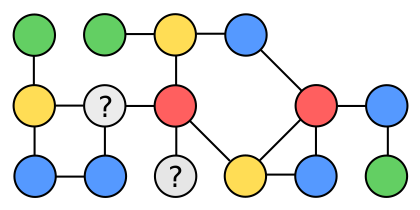
\includegraphics[width=0.4\linewidth]{images/VertexClassificationExample}
	\caption{Example of a graph with colors as vertex features.}
	\label{fig:vertexclassificationexample}
\end{figure}
A closer look reveals that, in this example, the color of a vertex corresponds to its degree. Thus $\text{deg}(v)$ may be a simple representation of each vertex $v$.

\paragraph{Example - Graph classification:} Consider the graph depicted in Figure \ref{fig:graphclassificationexample} and the task to predict the class of an unclassified graph (e.g. the gray one in the figure).
\begin{figure}[H] %TODO: Is this image TeXed? Lecture 0 Slide 30
	\centering
	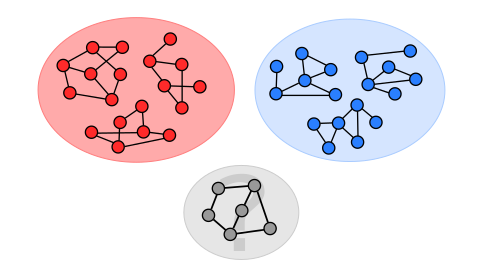
\includegraphics[width=0.5\linewidth]{images/GraphClassificationExample}
	\caption{Example of graph classification (clustering).}
	\label{fig:graphclassificationexample}
\end{figure}
A common approach is to use sets of subgraphs to describe (similarity between) graphs. In this example it appears that graphs of the red class contain cycles of length four whereas graphs of the blue class contain triangles. Thus, a graph $G$ may be represented by a vector $\phi(G)$ containing cycle counts of length three and four. 

\paragraph{Example - Link prediction:} Consider the graph depicted in Figure \ref{fig:linkpredictionexample} and the task to predict the likelihood of a not jet existing edge (e.g. the gray one in the figure).
\begin{figure}[H] %TODO: Is this image TeXed? Lecture 0 Slide 30
	\centering
	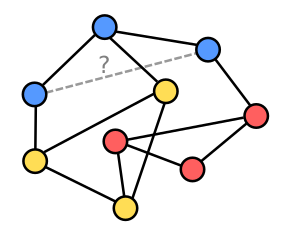
\includegraphics[width=0.4\linewidth]{images/LinkPredictionExample}
	\caption{Example of graph classification (clustering).}
	\label{fig:linkpredictionexample}
\end{figure}
A common approach is to consider the shortest path distance and similarity in terms of neighborhoods or vertex attributes. In this example the vertices of same color are more likely to be connected by an edge. Thus one may represent edges using the adjacent vertex colors.


As the given examples indicate, it can be tedious to analyze graph data and choose a suitable graph representation. As it turns out, Machine Learning can be used for learning the graph representations themselves. In the following chapter we will cover two aspects of graph representation learning:\begin{itemize}
	\item \textbf{Learning with representations} of graphs and
	\item \textbf{learning representations} of graphs.
\end{itemize}

%%%%%%%%%%%%%%%%%%%%%%%%%%%%%%%%%%
%%%%% Lecture 01 - 18.10.2021 %%%%
%%%%%%%%%%%%%%%%%%%%%%%%%%%%%%%%%%

\chapter{Vertex classifications and local features}

\begin{Definition}[Directed graph]{def:DirectedGraph}
	A \textbf{directed graph} (\textbf{digraph}) $G=(V,E)$ consists of a set of vertices $V(G)$ and a set of edges $E(G) \subseteq V\times V$.
\end{Definition}

\begin{Definition}[Undirected Graph]{def:UndirectedGraph}
	A \textbf{undirected graph} $G=(V,E)$ consists of a set of vertices $V(G)$ and a set of edges $E(G) \subseteq 2^V$ such that
	\[ \forall e\in E(G):\qquad |e|=2 \]
\end{Definition}

As variable naming conventions, we say that graphs have $n=|V(G)|$ vertices and $m=|E(G)|$ edges.

\begin{Definition}[Simple graphs]{def:SimpleGraph}
	A simple graph is a graph, where edges connot appear multiple times.	
\end{Definition}

(That is, in the respective definitions of directed and undirected graphs, the set of edges is not a multiset.)

\begin{Definition}[Graph attributes and labels]{def:GraphAttributesLabels}
	Given an undirected or directed graph $G$, one can define additional data associated with the graph, vertices or edges. Such data is called \textbf{attributes} (if the value domain is continuous) or \textbf{labels} (if the value domain is discrete/categorical).
	
	This association can be formalized using \textbf{feature spaces} $\mathcal{X}^G$, $\mathcal{X}^V$ and $\mathcal{X}^E$:
	\[ f_G(G) \to \mathcal{X}^G,\qquad\qquad f_V\big(V(G)\big) \to \mathcal{X}^V,\qquad\qquad f_E\big(E(G)\big) \to \mathcal{X}^E\]
	(A feature space is some product space $\mathcal{X}=(X_1,X_2,\dots,X_d)$ where the $X_i$ are some appropriately chosen sets.)
\end{Definition}

\paragraph{Example - Graph labels} Typical examples of graph vertex labels are atom names (chemical graphs).

\begin{Definition}[Graph isomorphism]{def:GraphIsomorphism}
	Let $G$ and $H$ be two graphs. $G$ and $H$ are \textbf{isomorphic}, if and only if there exists a bijective function between the vertices $\varphi:V(G)\to V(H)$ such that
	\begin{itemize}
		\item edges are preserved:\\
		$ \{v,w\}\in E(G) \ \iff \ \{\varphi(v), \varphi(w)\}\in E(H) $
		\item vertex attributes are preserved:\\
		$ \forall v\in V(G):\ f_V(v) = f_V\big( \varphi(v)\big) $
		\item edge attributes are preserved:\\
		$ \forall \{v,w\}\in E(G):\ f_E(\{v,w\}) = f_E\big( \{ \varphi(v),\varphi(w) \} \big) $
	\end{itemize}
\end{Definition}

\section{Property prediction for vertices}

Learning functions (properties) on vertices is done under the assumption that there is a multiset of objects $X\subseteq \mathcal{X}$ and there exists an (partially) unknown function $y:X\to \mathcal{Y}$ and some pairs of objects are associated. This setting is formalized in definition \ref{def:SupervisedVPropPredition}.

\begin{Definition}[Supervised vertex property prediction on fixed graphs]{def:SupervisedVPropPredition}
	\vspace{-0.5cm}\begin{tabbing}
		\textbf{Output:} \= \kill
		\textbf{Input:} \>a graph $G$ with labeling functions $f_V$, $f_E$,\\
		\>a hypothesis class $\mathcal{H} \subseteq\{ h|\ h:V(G)\to \mathcal{Y} \}$,\\
		\>properties $y(v)$ for a set of vertices $v\in V^\prime \subseteq V(G)$ and\\
		\>a loss function $L_{V,y}:\mathcal{H}\to\IR$.\\
		\textbf{Output:} \>$\amin{h\in\mathcal{H}}{L_{V,y}}(h)$.
	\end{tabbing}
\end{Definition}

Note that one can extend hypothesis classes on graph vertices to their vertex representation. More explicitly, let $\mathcal{X}$ be a feature space and $r:V(G)\to \mathcal{X}$ some vertex representation on the graph $G$. Let $\mathcal{H}\subseteq \{ h|\ h:\mathcal{X}\to\mathcal{Y} \}$ be a hypothesis class. Then the \textit{extended hypothesis class} 
\begin{equation}
	\mathcal{H}^\prime := \{ h\circ r|\ h\in\mathcal{H} \}
\end{equation}
is a hypothesis class on $V(G)$, too.

On top of that one can generalize the vertex representation $r$ to a set of several graph representation $\mathcal{R}\subseteq \{r|\ r:V(G)\to\mathcal{X}\}$ and yield the further extended hypothesis class $\mathcal{H}^\prime := \{ h\circ r|\ r\in\mathcal{R},\ h\in\mathcal{H} \}$ on $V(G)$.

\subsection{Loss Functions - MERGE \& MOVE WITH THE STATISTIC SCRIPT} %TODO: MOVE TO THE STATISTIC SCRIPT

To measure the quality of hypothesis, with respect to vertex property predictions, one can use a variety of loss functions. Most of these can be generalized to other applications of hypothesis evaluation.

\begin{Definition}[Classification Loss]{def:ClassificationLoss}
	The \textbf{classification loss} of a hypothesis on vertices to predict their properties is defined as the probability of false predictions:
	\begin{equation}
		L_{V,y}(h) := \IP\big[ y(v) \neq h(v) \big] = 1-\frac{1}{|V(G)|} \sum_{v\in V(G)}\delta \big( y(v), h(v) \big)
	\end{equation}
	where 
	\[ \delta(a, b) = \begin{cases}
	1 & \text{if } a=b\\
	0 & \text{if } a\neq b
	\end{cases} \]
\end{Definition}

\begin{Definition}[Regression]{def:Regression}
	The \textbf{mean squared error} can be used as a loss function of a hypothesis on vertex property prediction. Using it to improve the quality of the found hypothesis is called \textbf{regression}:
	\begin{equation}
		L_{V,y}(h) := \IE\Big[ \big( y(x) -h(x)\big)^2 \Big] = \frac{1}{|V(G)|} \sum_{v\in V(G)} \big( y(v), h(v) \big)^2
	\end{equation}
\end{Definition}

When evaluating a (machine learning) model during training, we test a hypothesis on empirical data and optimize for the best solution. Both the optimization and the empirical data induce a bias on the estimate of the quality of the hypothesis. This bias can be reduced using \textbf{cross validation} (TODO - see Figure \ref). %TODO

\begin{figure}[H]
	\centering
	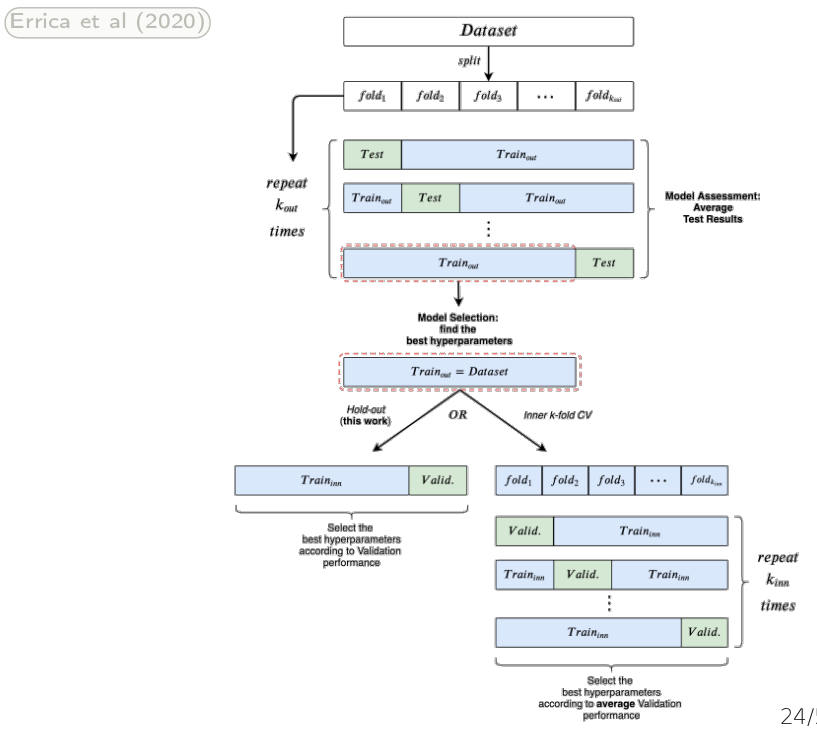
\includegraphics[width=0.7\linewidth]{images/crossvalidation}
	\caption{TODO: replace image} %TODO: replace image
	\label{fig:crossvalidation}
\end{figure}

Cross validation can be used to compare different hypothesis. If there is a statistically significant difference between their performances, one could be better than the other.

\subsection{Baselines for graph learning}

Interestingly, some baseline methods, which do not include specific graph structures may perform well, even better than GNNs on some graph datasets. In other words, improvements that do not clearly outperform structure-agnostic competitors should be viewed with moderation.

Note that whenever information about individual vertices is available, one should consider using it extensively. In many cases, it is more valuable for the task at hand, than the actual graph structure that combines these. 

To conclude, to evaluate a graph representation one should measure its performance against a model which ignores the graph structure. Thus when dealing with an attributed graph $G$ it can be beneficial to start with its vertex attributes $f_V: V(G)\to\mathcal{X}$ and first consider a hypothesis class over $\mathcal{X}$, only. Only after that, one may think about including graph representations into the hypothesis class.

\subsection{Local Feature Counts}

In this subsection we will define various simple vertex representations $f:V(G)\to\IR$ for fixed graphs. Let $\mathcal{R}^\prime$ be the set of all one-dimensional vertex representations. These representations can be grouped in the following way:
\begin{equation}
	\mathcal{R} := \{\times_R:V(G)\to\IR^{|R|}| \ R\subseteq \mathcal{R}^\prime\}
\end{equation}
where $\times_R(v)=\big( r_1(v), r_2(v),\dots, r_{|R|}(v) \big)$ for a vertex $v$ and representations $r_i\in R$.

\begin{Definition}[Vertex neighborhood]{def:VertexNeighborhood}
	Let $G$ be a undirected graph and $v\in V(G)$. The \textbf{neighborhood} of $v$ is the set
	\[ N(v):= \{w|\ \{v,w\}\in E(G)\} \]
	
	If $G$ is directed, we define respectively the \textbf{outgoind neighborhood} as 
	\[ N_{\text{out}}(v):= \{w|\ (v,w)\in E(G)\} \]
	and the \textbf{incoming neighborhood} as
	\[ N_{\text{in}}(v):= \{w|\ (w,v)\in E(G)\} \]
\end{Definition}

\begin{Theorem}[Full Neighborhood Representation]{thm:FullNeighborhoodRepresentation}
	By fixing an order of the vertices $V=\{ v_1,\dots,v_n \}$ and defining 
	\begin{equation}
	A(v_j)[i] :=\begin{cases}
	1 & \text{if }v_i\in N(v_k)\\
	0 & \text{if }v_i\notin N(v_k)
	\end{cases}
	\end{equation}
	one can represent a vertex by its neighborhood. This is called \textbf{Full Neighborhood Representation}.
\end{Theorem}

The drawbacks of a Full Neighborhood Representation include:\begin{itemize}
	\item The space requirements grow quadratically with $n$.
	\item Learning algorithms that use this representation will likely overfit.
	\item It requires additional effort to check, whether a given vertex is already included in the representation.
	\item It requires additional effort to find neighbors of neighbors.
\end{itemize}

The first two drawbacks can be reduced, by so called Compressed Neighborhood Representations. 

\begin{Definition}[Vertex degree]{def:VertexDegree}
	Let $G$ be a undirected graph and $v\in V(G)$ be a vertex. The \textbf{degree} is the number of edges incident to $v$, i.e.
	\[ \delta(v) := |N(v)| \]
	
	if $G$ is directed, we define respectively the \textbf{outdegree neighborhood} as the number of (incident) edges starting in $v$, i.e. 
	\[ \delta_{\text{out}}(v) := |N_{\text{out}}(v)| \]
	and the \textbf{indegree neighborhood} as the number of (incident) edges ending in $v$, i.e. 
	\[ \delta_{\text{out}}(v) := |N_{\text{out}}(v)| \]
\end{Definition}

The neighborhood $N(v)$ of a vertex $v$ induces a subgraph $G[N(v)]$ with the vertices in $N(v)$ and all edges between these vertices:
\[ G[N(v)] = \Big( N(v), \big\{\{w,w^\prime\}|\ w,w^\prime\in N(v) \big\} \Big) \]
The generalized definition is given in definition \ref{def:InducedSubgraph}.
This subgraph $G[N(v)]$ can have at most
\[ \frac{\delta(v)\big( \delta(v)-1 \big)}{2} \]
edges, since every of the $\delta(v)$ neighbors of $v$ can have at most one edge, to all other $\delta(v)$ neighbors in $G[N(v)]$. Notice, not to count every edge twice in this argumentation. If there are exactly this many edges (without loops), the subgraph is \textit{fully connected}.

\begin{Definition}[Neighborhood density]{def:NeighborhoodDensity}
	The \textbf{density} of a vertex's neighborhood $v$ is defined as the ratio of all existing edges and all possible edges (in a fully connected neighborhood):
	\[ c(v) := \frac{2 \big|E\big( G[N(v)] \big)\big|}{ \delta(v) \big(\delta(v)-1\big) } \]
\end{Definition}

\begin{Definition}[Induced subgraph]{def:InducedSubgraph}
	Let $G$ be a graph and $X\subseteq V(G)$ a set of its vertices. The \textbf{subgraph} of $G$ \textbf{induced by} $X$ is the graph $H$ with \begin{itemize}
		\item $V(H) = X$ and
		\item $E(H) = \big\{ \{v,w\}|\ \{v,w\}\in E(G)\ \land \ v,w\in X \big\}$
	\end{itemize}
\end{Definition}

A \textbf{triangle graph} is a simple graph on three vertices with three edges. 

\begin{Definition}[Triangle subgraphs]{def:TriangleSubraphCount}
	Let $\mathcal{D}(v)$ be the set of all triangle subgraphs of a graph $G$ that contain the vertex $v$.
	
	Let $\Delta(v) := |\mathcal{D}(v)|$ be its carnality.
\end{Definition}

\begin{Theorem}[Upper bound on the adjacent triangle count]{thm:AdjacentTriangleCount}
	Let $G$ be a graph and $v\in V(G)$. Then
	\[ \Delta(v) \le \big|E(G[N(v)])\big| \]
\end{Theorem}
\begin{Proof}
	Let $D\in\mathcal{D}(v)$ be an arbitrary triangle adjacent to $v \in V(G)$. Then $V(D) \subseteq N(v) \subseteq G[N(v)]$ since in a triangle all vertices are adjacent and thus all vertices in the triangle are adjacent to $v$ (i.e. contained in its neighborhood).
	
	Notice, that there are two kind of edges in $G[N(v)]$, the ones incident to $v$ ($v\in e$, there are $\delta(v)$ many of them) and these which are not ($v\notin e$). The ones incident to $v$ can be part of at most two triangles in $\Delta(v)$, while the edges that are not incident to $v$ can be part in exactly one triangle in $\Delta(v)$. That is because the two vertices that are adjacent to such an edge, together with $v$, completely define a triangle (if all edges are present).
	On the other hand, every triangle in $D(v)$ must contain exactly one edge, that is not incident to $v$ (and two which are incident to $v$).
	
	Therefore the number of triangles $\Delta(v)$ is equal to the number of edges in $G[N(v)]$ that are not incident to $v$, which is a fraction of all edges in $G[N(v)]$:
	\begin{flalign*}
		\Delta(v) &= \big|\{ e\in E(G[N(v)])| \ v\notin e\}\big| \\
		&\le \big|\{ e\in E(G[N(v)])| \ v\notin e\}\big| + \delta(v)\\
		&= \big|E(G[N(v)])\big|
	\end{flalign*}
	(Note that in the second equation, the equality is only achieved, if $v$ has no neighbors.)
\end{Proof}

\begin{Definition}[Induced Subgraph Isomorphism Problem]{def:InducedSubgraphIsoPb}
	\vspace{-0.5cm}\begin{tabbing}
		\textbf{Output:} \= \kill
		\textbf{Input:} \>two graphs $G$, $H$.\\
		\textbf{Output:} \>the decision if $H$ is isomorphic to an induced subgraph of $G$.
	\end{tabbing}
\end{Definition}

\begin{Theorem}[Difficulty of the Ind. Subgraph Iso. Pb.]{def:NPCompletenessOfInducedSubgraphIsoPb}
	The induced subgraph isomorphism problem is \textbf{NP-complete}.
\end{Theorem}
\begin{Proof}
	Let $K_n$ be a complete graph on $n$ vertices. Then solving the induced subgraph isomorphism problem for $K_n$ and $G$ solves the $k$-Clique Problem for $G$, which is NP-complete itself.
\end{Proof}

Notice, that if one could count the induced subgraphs for two graphs efficiently, one could decide the induced subgraph isomorphism problem. Hence \textit{counting induced subgraphs is NP-hard}.

But if one keeps the size of the induced subgraphs fix, the problem becomes tractable. 

\subsection{Graphlet Counting}

\begin{Definition}[Graphlet]{def:Graphlet}
	Small connected induced subgraphs are called \textbf{graphlets}.
\end{Definition}

We would like to count, for each vertex $v$, the number of graphlets of a certain type, that contain $v$. Lets call these $v$\textbf{-incident graphlets}.

\begin{Definition}[Incident Induced Graphlets Count Problem]{def:InducedSubgraphIsoPb}
	\vspace{-0.5cm}\begin{tabbing}
		\textbf{Output:} \= \kill
		\textbf{Input:} \>a graph $G$ and\\ 
		\>a graphlet $H$ of size $k$.\\
		\textbf{Output:} \>the number of $v$-incident induced subgraphs isomorphic to $H$ for all $v\in V(G)$:\\
		\>$ r_H(v) := \big|\{ X\subseteq V| \ v\in X\ \land\ G[X] \stackrel{\text{iso.}}{\equiv} H \}\big| $
	\end{tabbing}
\end{Definition}

\begin{algorithm}[H]
	\caption{Brute Force - Counting Incident Graphlets} \label{alg:BruteForceCountingIncidentGraphlets} 
	\begin{tabbing}
		\textbf{Output:} \= \kill
		\textbf{Input:} \>a graph $G$ and\\ 
		\>a graphlet $H$ of size $k$.\\
		\textbf{Output:} \>the number of $v$-incident induced subgraphs isomorphic to $H$ for all $v\in V(G)$.
	\end{tabbing}	
	\begin{algorithmic}[1]		
		\State $\text{gc}(v)=0$ for all $v\in V(G)$
		\For {\textbf{all} $X\subseteq V(G)$ with $|X|=k$}
			\If{$G[X]$ is isomorphic to $H$}
				\State Increment $\text{gc}(x)$ for all $x\in X$
			\EndIf
		\EndFor
	\end{algorithmic}
	\textbf{Runntime}: There are ${n\choose k}$ choices for $X$, and there need $\gamma(k)\in \mathcal{O}( k! \ k^2)$ graphs to be checked for isomorphism. Thus the total runtime for a constant $k$ is
	\[ \mathcal{O} \big( n^k \ \gamma(k) \big) = \mathcal{O}(n^k)\]	
\end{algorithm}

Since a lot of graph structured data can be considered Big Data (w.r.t. size; not speed), cubic runtime in the number of vertices is not acceptable.

\begin{Theorem}[Runtime bound on the Incident Induced Graphlets Count Problem]{thm:RuntimeBoundIncIndGraphletsCountPb}
	Let $G$ be a bounded degree graph and let $d$ denote the maximum degree in $G$. Then all $v$-incident graphlets of $G$ with size $k\in \{ 3, 4, 5 \}$ can be enumerated in $\mathcal{O}(nd^{k-1})$ time.
\end{Theorem}
Notice that the maximum degree $d$ of a graph is typically much smaller than the number of its vertices $n$.
\begin{Proof}
	Graphlets of size $k$ can be divided into two classes:\begin{itemize}
		\item Graphlets that contain a simple path of length $k-1$ and
		\item Graphlets that to not contain such a path.
	\end{itemize}
	%TODO: CONTINUE - Slide 14/59
\end{Proof}

%%%%%%%%%%%%%%%%%%%%%%%%%%%%%%%%%%
%%%%% Lecture 02 - 25.10.2021 %%%%
%%%%%%%%%%%%%%%%%%%%%%%%%%%%%%%%%%



\chapter{Announced Topics}
\section{Link prediction}



\section{Graph classification, regression and clustering in transactional graph databases}


\chapter{Feature Extraction and Graph Mining}

In this chapter we focus on extracting graph representations following a fixed process. Therefore we discuss several pattern (or feature) classes and focus on the following questions:
\begin{itemize}
	\item What kind of features are there (e.g. local and global)?
	\item How viable are these features?
	\item How expressive is their extraction?
	\item How powerful are graph representations in terms of distinguishing inputs?
	\item How do we evaluate their quality?
\end{itemize}

\chapter{Learning on Graphs and Graph Kernels}

In this chapter we discuss learning with (implicit) graph representations. Therefore we introduce machine learning models specific to the task of classifying graphs.

\section{Support Vector Machine (SVM)}
\section{Expressive power of machine learning models}
\section{Kernel of special interest: Weisfeiler-Lehman kernel}

\chapter{Graph Neural Networks (GNNs)}

In this chapter we will introduce the learning of representations of graphs. We discuss how neural networks can be used to learn graph representations and to subsequently perform machine learning tasks.

\section{Relationship to Weisfeiler-Lehman method}
\section{Structure of GNNs}
\section{Expressive power of GNNs}




%%%%%%%%%%%%%%%%%%%%%%%%%%%%%%%%%%
%%%%% Lecture 03 - dd.mm.2021 %%%%
%%%%%%%%%%%%%%%%%%%%%%%%%%%%%%%%%%

%%%%%%%%%%%%%%%%%%%%%%%%%%%%%%%%%%
%%%%% Lecture 04 - dd.mm.2021 %%%%
%%%%%%%%%%%%%%%%%%%%%%%%%%%%%%%%%%

%%%%%%%%%%%%%%%%%%%%%%%%%%%%%%%%%%
%%%%% Lecture 05 - dd.mm.2021 %%%%
%%%%%%%%%%%%%%%%%%%%%%%%%%%%%%%%%%

%%%%%%%%%%%%%%%%%%%%%%%%%%%%%%%%%%
%%%%% Lecture 06 - dd.mm.2021 %%%%
%%%%%%%%%%%%%%%%%%%%%%%%%%%%%%%%%%

%%%%%%%%%%%%%%%%%%%%%%%%%%%%%%%%%%
%%%%% Lecture 07 - dd.mm.2021 %%%%
%%%%%%%%%%%%%%%%%%%%%%%%%%%%%%%%%%

%%%%%%%%%%%%%%%%%%%%%%%%%%%%%%%%%%
%%%%% Lecture 08 - dd.mm.2021 %%%%
%%%%%%%%%%%%%%%%%%%%%%%%%%%%%%%%%%

%%%%%%%%%%%%%%%%%%%%%%%%%%%%%%%%%%
%%%%% Lecture 09 - dd.mm.2021 %%%%
%%%%%%%%%%%%%%%%%%%%%%%%%%%%%%%%%%

%%%%%%%%%%%%%%%%%%%%%%%%%%%%%%%%%%
%%%%% Lecture 10 - dd.mm.2021 %%%%
%%%%%%%%%%%%%%%%%%%%%%%%%%%%%%%%%%

%%%%%%%%%%%%%%%%%%%%%%%%%%%%%%%%%%
%%%%% Lecture 11 - dd.mm.2021 %%%%
%%%%%%%%%%%%%%%%%%%%%%%%%%%%%%%%%%

%%%%%%%%%%%%%%%%%%%%%%%%%%%%%%%%%%
%%%%% Lecture 12 - dd.mm.2021 %%%%
%%%%%%%%%%%%%%%%%%%%%%%%%%%%%%%%%%

%%%%%%%%%%%%%%%%%%%%%%%%%%%%%%%%%%
%%%%% Lecture 13 - dd.mm.2021 %%%%
%%%%%%%%%%%%%%%%%%%%%%%%%%%%%%%%%%

%%%%%%%%%%%%%%%%%%%%%%%%%%%%%%%%%%%%%%%%%%%%%%%%%%%%%%%%%%%%%%%%%%%%%%%%%%%%%%%%%%%%%%%%%%%%%%%

\newpage
%%%% ----------------------- %%%%
%%%% -------Exercises------- %%%%
%%%% ----------------------- %%%%

% !TeX spellcheck = en_GB 

\chapter{Exercises}
\section{Sheet 0 - Python}

\newpage
\section{Sheet 1}

\subsection{Assignment 1a - Bias of an estimator} 
\dots
\paragraph{Solution:} 
\begin{minipage}{\textwidth}
	\begin{minipage}[b]{0.49\textwidth}
		\begin{figure}[H]
			\centering
			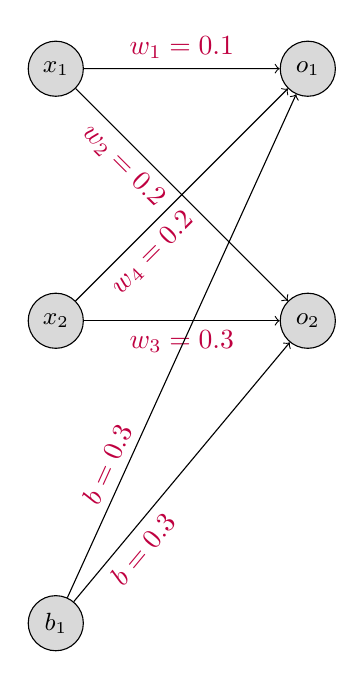
\begin{tikzpicture}[x=2cm,y=2cm] 
			\begin{scope}[scale=1.6]
			
			\tikzstyle{mycircle}=[circle,
			draw=black,
			fill=gray,
			fill opacity = 0.3,
			text opacity=1,
			inner sep=0pt,
			minimum size=7mm,
			font=\small
			]
			\tikzstyle{myline}=[-]
			\tikzstyle{myarrow}=[->]
			
			\coordinate (px1) at (-1, 1);
			\coordinate (px2) at (-1, 0);
			\coordinate (pb1) at (-1, -1.2);
			
			\coordinate (po1) at (0, 1);
			\coordinate (po2) at (0, 0);
			
			
			\node[mycircle] (x1) at (px1) {$x_1$};	
			\node[mycircle] (x2) at (px2) {$x_2$};	
			\node[mycircle] (b1) at (pb1) {$b_1$};	
			
			\node[mycircle] (o1) at (po1) {$o_1$};	
			\node[mycircle] (o2) at (po2) {$o_2$};	
			
			\draw[myarrow] (x1) -- node[purple, auto] {$w_1=0.1$} (o1);			
			\draw[myarrow] (x1) -- node[purple, sloped, anchor=x2, below left] {$w_2=0.2$} (o2);
			
			\draw[myarrow] (x2) -- node[purple, below] {$w_3=0.3$} (o2);			
			\draw[myarrow] (x2) -- node[purple, sloped, anchor=x2, below left] {$w_4=0.2$} (o1);
			
			
			\draw[myarrow] (b1) -- node[purple, sloped, above, near start] {$b=0.3$} (o1);
			\draw[myarrow] (b1) -- node[purple, sloped, below, near start] {$b=0.3$} (o2);
			
			\end{scope}
			\end{tikzpicture}
		\end{figure}
		\captionof{figure}{Multi-Layer Perceptron}
		\label{fig:Sheet5Ex1}
	\end{minipage}
	\hfill
	\begin{minipage}[b]{0.49\textwidth}
		\centering
		\begin{tabular}{ |c | c | c | c | c |}
			\hline
			$n$ & $x_1$ & $x_2$ & $p_1$ & $p_2$\\ \hline
			$1$ & $0.1$ & $0.4$ & $0.1$ & $0.9$\\ \hline
			$2$ & $0.8$ & $0.2$ & $0.95$ & $0.05$\\ \hline
			$3$ & $0.6$ & $0.5$ & $0.4$ & $0.6$\\ \hline
			$4$ & $0.3$ & $0.9$ & $0.75$ & $0.25$\\ \hline
			$5$ & $0.3$ & $0.5$ & $0.9$ & $0.1$\\ \hline
		\end{tabular}
		\captionof{table}{Training batch}
	\end{minipage}
\end{minipage}

\begin{algorithm}[H] 
	\caption{Generative Adversarial Networks (GAN)}%\label{alg:GAN}
	\begin{tabbing}
		\textbf{Output:} \= \kill
		\textbf{Input:} \> a discriminator function $D$,\\
		\> a generator function $G$,\\
		\> noise samples $Z$,\\
		\> true samples $X$ (with an underlying data generation distribution $\IP_{\text{data}}[X]$),\\
		\> desired size of mini-batches $m$,\\
		\> a number $k$ of improvement iterations for the discriminator,\\
		\> stopping criterion $T_{\text{condition}}$\\
		\textbf{Output:} \> a generator $G$ that is able to fool the trained discriminator $D$
	\end{tabbing}
	\begin{algorithmic}[1]
		\While {not $T_{\text{condition}}(f, \theta)$}
		\For {$k$ steps}
		\State Sample a minibatch of noise samples $\{z^{(1)}, \dots, z^{(m)}\}$
		\State Sample a minibatch of true samples $\{x^{(1)}, \dots, x^{(m)}\}$
		\State Perform stochastic gradient ascend for the discriminator:
		\[ \nabla_{\theta^{(d)}}\frac{1}{m}\sum\limits_{i=1}^{m}\Big( \log\big( d(x^{(i)};\theta^{(d)}) \big) + \log\big(1-d\big(g(z^{(i)};\theta^{(g)}),\theta^{(d)}\big)\big) \Big) \]
		\EndFor
		\State Sample a minibatch of noise samples $\{z^{(1)}, \dots, z^{(m)}\}$
		\State Perform stochastic gradient descending for the generator:
		\[ \nabla_{\theta^{(g)}}\frac{1}{m}\sum\limits_{i=1}^{m}\Big(  \log\big(1-d\big(g(z^{(i)};\theta^{(g)}),\theta^{(d)}\big)\big) \Big) \]
		\EndWhile
	\end{algorithmic}	
\end{algorithm}

\newpage
%%%% ----------------------- %%%%
%%%% ------Bibliography----- %%%%
%%%% ----------------------- %%%%
\begin{thebibliography}{4}

\bibitem[1]{1}
\glqq EXAMPLE: Finite Elemente - Theorie, schnelle L�ser und Anwendungen in der Elastizit�tstheorie \grqq von Dietrich Braess, 5. Auflage, Springer, 2013

\end{thebibliography}

\end{document}
